\subsection{EXTENSION OF THE RING OF SCALARS}

Let A, A' be two commutative rings and \(\rho:A\to A'\) a ring homomorphism. Let M be an A-module, M' an A'-module and \(u:M\to M'\) an A-homomorphism; as the canonical injection \(\phi_{M'}:M'\to T_{A'}(M')\) is also an A-homomorphism (by restriction of scalars), so is the composition \(M\xrightarrow{u}M'\xrightarrow{\phi_{M'}}T_{A'}(M')\) . An A-algebra homomorphism \(T_{A}(M)\to\rho*(T_{A'}(M'))\) is derived (no. 2), also denoted by \(T(u):T_{A}(M)\to T_{A'}(M')\) , which is the unique A-homomorphism rendering commutative the diagram

\begin{enumerate}
\def\labelenumi{(\arabic{enumi})}
\setcounter{enumi}{7}
\tightlist
\item
\end{enumerate}

\pandocbounded{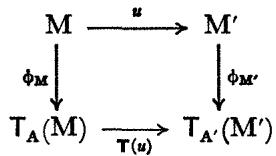
\includegraphics[keepaspectratio]{images/part003_9672ae23.jpg}}

If \(\sigma: \mathbf{A}' \to \mathbf{A}''\) is a commutative ring homomorphism, \(\mathbf{M}''\) an \(\mathbf{A}''\) -module and \(v: \mathbf{M}' \to \mathbf{M}''\) an \(\mathbf{A}'\) -homomorphism, the above uniqueness property shows that

\[
\mathbf {T} (v \circ u) = \mathbf {T} (v) \circ \mathbf {T} (u).\tag{9}
\]

PROPOSITION 5. Let A, B be two commutative rings, \(\rho: \mathbf{A} \to \mathbf{B}\) a ring homomorphism and M an A-module. The canonical extension

\[
\psi : \mathsf {T} _ {\mathbf {B}} (\mathbf {B} \otimes_ {\mathbf {A}} \mathbf {M}) \rightarrow \mathbf {B} \otimes_ {\mathbf {A}} \mathsf {T} _ {\mathbf {A}} (\mathbf {M})
\]

of the B-linear mapping \(\mathbf{1}_{\mathbf{B}} \otimes \phi_{\mathbf{M}}: \mathbf{B} \otimes_{\mathbf{A}} \mathbf{M} \to \mathbf{B} \otimes_{\mathbf{A}} \mathsf{T}_{\mathbf{A}}(\mathbf{M})\) is an isomorphism of graded B-algebras.

Consider the two A-algebra homomorphisms: the canonical injection \(j: \mathbf{B} = \mathsf{T}^0(\mathbf{B} \otimes_{\mathbf{A}} \mathbf{M}) \to \mathsf{T}(\mathbf{B} \otimes_{\mathbf{A}} \mathbf{M})\) and the homomorphism

\[
h = \mathsf {T} (i): \mathsf {T} (\mathbf {M}) \rightarrow \mathsf {T} (\mathbf {B} \otimes_ {\mathbf {A}} \mathbf {M})
\]

derived (cf.~formula (8)) from the canonical A-linear mapping

\[
i: \mathbf {M} \rightarrow \mathbf {B} \otimes_ {\mathbf {A}} \mathbf {M}.
\]

As \(\mathsf{T}^0 (\mathbf{B}\otimes_{\mathbf{A}}\mathbf{M})\) is contained in the centre of \(\mathsf{T}(\mathbf{B}\otimes_{\mathbf{A}}\mathbf{M})\) , Proposition 5 of §4, no. 2 can be applied and an A-algebra homomorphism

\[
\psi^ {\prime}: \mathbf {B} \otimes_ {\mathbf {A}} \mathsf {T} (\mathbf {M}) \rightarrow \mathsf {T} (\mathbf {B} \otimes_ {\mathbf {A}} \mathbf {M})
\]

is obtained such that, for \(\beta \in \mathbf{B}\) , \(x_{i} \in \mathbf{M}\) for \(1 \leqslant i \leqslant n\) ,

\[
\psi^ {\prime} (\beta \otimes (x _ {1} \otimes x _ {2} \otimes \dots \otimes x _ {n})) = \beta ((1 \otimes x _ {1}) \otimes (1 \otimes x _ {2}) \otimes \dots \otimes (1 \otimes x _ {n})),
\]

which shows immediately that \(\psi'\) is also a B-algebra homomorphism. It suffices to prove that \(\psi \circ \psi'\) and \(\psi' \circ \psi\) are the identity mappings on \(B \otimes_{A} T(M)\) and \(T(B \otimes_{A} M)\) respectively. Now, these two algebras are generated by \(B \otimes_{A} M\) and clearly \(\psi \circ \psi'\) and \(\psi' \circ \psi\) coincide with the identity mapping on \(B \otimes_{A} M\) , whence the conclusion.

